\chapter{Testing}

% Detailed descriptions of every test case are definitely not what is required here. What is important is to show that you adopted a sensible strategy that was, in principle, capable of testing the system adequately even if you did not have the time to test the system fully.

% Have you tested your system on �real users�? For example, if your system is supposed to solve a problem for a business, then it would be appropriate to present your approach to involve the users in the testing process and to record the results that you obtained. Depending on the level of detail, it is likely that you would put any detailed results in an appendix.

% The following sections indicate some areas you might include. Other sections may be more appropriate to your project. 

\section{Overall Approach to Testing}
My approach to testing was using Test Driven Development and refactoring, taking note from XP practices, ensuring that I only developed as muchas was required to make tests pass based upon my requriements for each bit of functionality. The aim was to have as many tests automated as possible, as this would allow me to test frequently and reliably and tie into testing everytime I checked into my Git repository with CodeShip's continuous integration of my code. Where automation could not be carried out, I created test files and used a test table to determine whether my application met the requirements I could test against.

%=== Up to here ===

\section{Automated Testing}
\subsection{Unit Tests}
Writing unit tests first to match against was very useful, allowing me to develop code againsts the tests, written one by one, so that I would not develop any more than necessary, and what was developed fit the requirements to be tested against. Refactoring the code after each test kept my design evolving and improving maintainability and simplicity to remove duplicate and unnecessary code.

\begin{figure}[H]
\centering
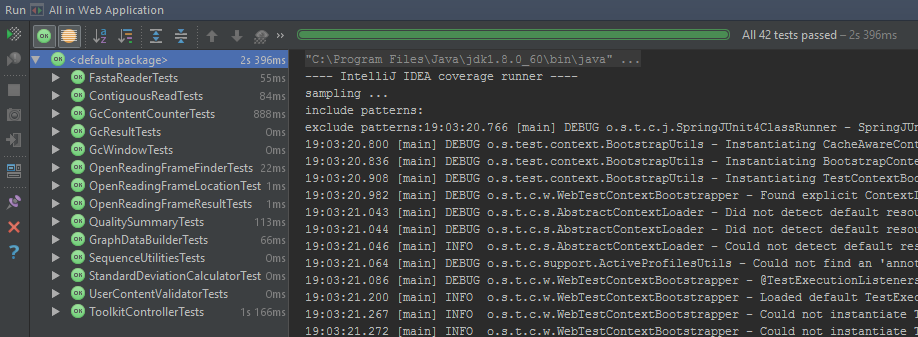
\includegraphics[width=0.9\textwidth]{images/unittestsuccess}
\caption{Results of running the set of unit tests developed for the application.}
\end{figure}

IntelliJ gave  me the tools to run my unit tests with coverage, allowing me to see how much of my code was actually tested against. In the figure below it can be seen that most of my methods were covered. Those methods that were not covered I chose not to test against, as they are mostly setters and getters with no further functionality. In practice, it would perhaps be best to test against these too, in case for some reason the way a value is set or retrieved had to take into account some processing.

\begin{figure}[H]
\centering
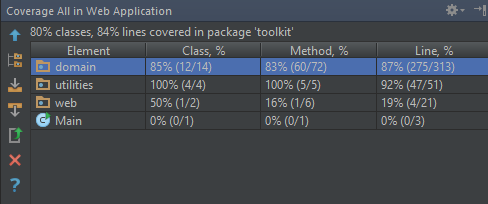
\includegraphics[width=0.9\textwidth]{images/testcoverage1}
\caption{The test coverage of my unit tests over the developed application code.}
\end{figure}

\begin{figure}[H]
\centering
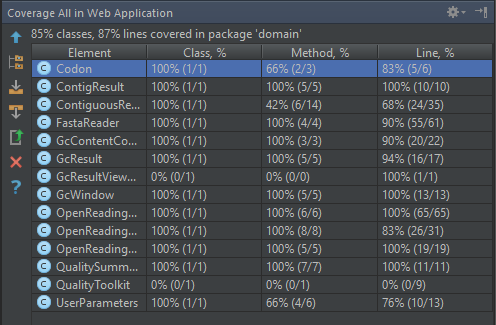
\includegraphics[width=0.9\textwidth]{images/testcoverage2}
\caption{The test coverage of my unit tests over the developed application code, broken down for each class.}
\end{figure}

%== Insert example of test here

\subsection{Integration Testing}
Testing of reading in files. Just asserting the data is as expected, and what happens with blank files, or erronous data files. Does the system handle it gracefully? (Show examples of those test files and what happens with bad files)

%=== Insert example of test here

\subsection{User Interface Testing}
Tested to see that it worked using Chrome's Developer Tools utility, testing in Chrome, Firefox and Microsoft Edge. (screenshots of how each page looks for each, including results and charts). Used YSoSlow to test page load speed
%== Show developer console here 
%== Show YSoSlow screenshot here


\subsection{Manual Testing}
A number of artificial test files were also created in order to be used for testing. Some of these were used in automated tests, such as checking for a files existence and possibility of being read, or throwing exceptions when a test file did not exist. Some files were for running manually, either being entirely artificial and checking for individual expected behavours or composed of actual data from multiple species that I manually split and combined together to view the results of. The artificial file data is included in the appendices.

Testing via a test table (Provided test table) - Tested files with known content and expected results to see response. Tested by viewing what I expected to happen, backing this up with the test table e.g. Click to view information, expected graph results based on artifical test files
Set goal of dealing with large files. Tested with large files to see if the system could process them on my laptop. Could be expanded to deal with much larger files on a system that could handle larger data files with more memory. For my laptop though, dealt with the files fine, even if some took some time to process due to my laptops processing speed.
Pasting large amounts of data in a single contig file - Result and time to process file and then inspection time
Pasting large amounts of data spread across multiple contigs - Result and time to process file and then inspection time
